% $File: report.tex
% $Date: Fri Jun 21 10:16:23 2013 +0800
% $Author: wyx <ppwwyyxxc@gmail.com>

\documentclass[11pt,a4paper]{article}

\usepackage{fontspec,amsmath,amssymb,zhspacing,verbatim,minted,listings,zhmath}
\usepackage{titlesec, titletoc}
\usepackage{threeparttable}
\usepackage{enumerate}
\usepackage[hyperfootnotes=false,colorlinks,linkcolor=blue,anchorcolor=blue,citecolor=blue]{hyperref}
\usepackage[sorting=none]{biblatex}
%\usepackage[dvips]{graphicx}
\usepackage{subfigure}
\usepackage{indentfirst}
\usepackage{float}			% don't automatically change location of figure [H]
\usepackage{chngpage}		% use \changetext to change page size
\usepackage{caption}\captionsetup{hypcap=true}  % ref to jump to object instead of caption
\newfontfamily\zhfont[BoldFont=SimHei,ItalicFont=KaiTi_GB2312]{SimSun}
\lstset{keywordstyle=\color{blue!70}, commentstyle=\color{red!50!green!50!blue!50},frame=shadowbox,rulesepcolor=\color{red!20!green!20!blue!20},
basicstyle=\footnotesize\ttfamily}
\zhspacing
\setlength{\parindent}{2em}

\usepackage{fancyhdr}
\changetext{}{2.2cm}{-1.1cm}{-1.1cm}{}
\pagestyle{fancy}
\setlength{\headheight}{15.2pt}
\lhead[]{}\rhead[]{}
\fancyhead[C]{\emph{图形学大作业报告}}


%use cell in tabular
\newcommand{\tabincell}[2]{\begin{tabular}{@{}#1@{}}#2\end{tabular}}

%thick shline
\newlength\savewidth
\newcommand\shline{\noalign{\global\savewidth\arrayrulewidth\global\arrayrulewidth 1pt}
                   \hline
                   \noalign{\global\arrayrulewidth\savewidth}}


\renewcommand{\abstractname}{摘要}
\renewcommand{\contentsname}{目录}
\renewcommand{\tablename}{表}
\renewcommand{\figurename}{图}
\defbibheading{bibliography}{\section{References}}
\bibliography{refs.bib}
\newcommand{\figref}[1]{\hyperref[fig:#1]{图\ref*{fig:#1}}}
\newcommand{\secref}[1]{\hyperref[sec:#1]{\ref*{sec:#1}节}}
\newcommand{\tabref}[1]{\hyperref[tab:#1]{表\ref*{tab:#1}}}

% math function
\let\Oldsum\sum
\renewcommand{\sum}{\displaystyle\Oldsum}
\let\Oldprod\prod
\renewcommand{\prod}{\displaystyle\Oldprod}


\input{mint-defs.tex}

%\title{第一次仿真作业}
%\author{吴育昕\\(清华大学计算机系~北京~100084~ppwwyyxxc@gmail.com)}
%\date{January, 2012}

\begin{document}
%\fontsize{10pt}{\baselineskip}
%\selectfont
%\maketitle

%\begin{abstract}

	%{\bf 关键词}
%\end{abstract}

% File: title.tex
% Date: Thu Jun 20 18:49:41 2013 +0800
% Author: Yuxin Wu <ppwwyyxxc@gmail.com>

\newcommand{\HUGE}{\fontsize{29pt}{29pt}\selectfont}
\renewcommand{\today}{\number\year 年 \number\month 月 \number\day 日}
\begin{titlepage}

% 首行的位置往上调整。但vspace前面需要有东西才会起效。

\phantom{Start!}

\vspace{-1.7cm}

\begin{flushleft}

\emph{\Large 清华大学计算机系}\\[0.2cm]

\emph{\Large 计算机图形学基础}\\[5.2cm]

% Title

\hspace{3cm}{ \HUGE \bfseries 光线追踪及网格简化}\\[0.4cm]


\hspace{3cm} {\huge \bfseries 作业文档}

\end{flushleft}





\vfill



\begin{flushright}

{

%\setCJKmainfont{Adobe Kaiti Std}

% \pillar:使用一种统一的方法提高行高

\newcommand{\pillar}{ {\Huge \phantom{A}} }

\large

\begin{tabular}{lc}

\pillar 姓名 & 吴育昕\\\cline{2-2}

\pillar 学号 & 2011011271 \\\cline{2-2}

\pillar 班级 & 计14 \\\cline{2-2}

\pillar 邮箱 &ppwwyyxxc@gmail.com \\\cline{2-2}

\end{tabular}

}

\end{flushright}

\end{titlepage}

\titleformat*{\section}{\centering\Large\bf}
\tableofcontents

% File: intro.tex
% Date: Sat Jun 22 23:04:03 2013 +0800
% Author: Yuxin Wu <ppwwyyxxc@gmail.com>

\section{简介}
本程序是一个3D渲染程序.
选用Phong模型\cite{phong}作为局部光照模型,渲染3D场景.
支持平面、球、三角面片、三角网格(可从obj文件读入)几种几何对象,并可方便的扩展.
渲染支持软阴影,抗锯齿,景深,自定义纹理等功能, 并可对三角网格进行简化.
三角网格,全局渲染,网格简化均采用数据结构(KD树及堆)与多线程加速,效率很高.
同时,将渲染功能嵌入了图形界面,可以支持obj文件的预览及简化.

\subsection{依赖}
\begin{enumerate}
  \item 本程序用C++11编写,需要编译器支持C++11中的ranged loop, initializer list, type inference等语法,
    且需标准库包含\verb|std::shared_ptr, std::future|
    类.建议使用g++$ \ge$ 4.8 编译.

  \item OpenCV2 \footnote{\url{http://opencv.org}}

  \item ImageMagick \footnote{\url{http://www.imagemagick.org/script/index.php}}

\item Qt4  \footnote{\url{http://qt-project.org/}} (可选)
\end{enumerate}


\subsection{编译}
在\verb|src|目录中,使用\verb|make|命令和\verb|make gui|命令分别编译命令行程序与图形界面程序.

\subsection{使用}

\begin{enumerate}
    \item 命令行程序:
      直接运行,渲染一个演示场景. 可在\verb|main()|函数中选择不同的场景.

      程序调用opencv进行图像显示,显示时可通过键盘进行导航,导航方法见下表:
\begin{table}[H]
  \begin{tabular}{c|c}
    \shline
    \UArrow \DArrow& 屏幕以视点到其连线为轴旋转, \UArrow 顺时针\\
    \LArrow \RArrow & 围绕固定中心旋转视点\\
    \keystroke{h}\keystroke{j}\keystroke{k}\keystroke{l} & 视点及屏幕的平移 \\
    \keystroke{=}\keystroke{-} & 缩放\\
    \keystroke{>}\keystroke{<} & 固定视点旋转视角\\
    \keystroke{]}\keystroke{[} & 调节焦平面远近(景深模式下有用), \keystroke{]}调远\\
    \keystroke{s} & 保存当前图片至output.png\\
    \keystroke{p} & 输出当前视角信息\\
    \keystroke{q} \Esc & 退出\\
  \end{tabular}
  \centering
  \caption{场景导航快捷键\label{tab:navigate}}
\end{table}

      \item 图形界面程序:
        运行界面如\figref{gui}所示,
        运行后,通过open按钮选择obj文件,trace按钮渲染,smooth控制是否开启法向插值.
        其余按钮用于更改视角、渲染方式等参数,改变视角后重新trace即可生效.
        simplify按钮将obj模型按照给定的简化率进行简化,simplify rate表示简化后保留的面片所占比例.

\end{enumerate}

% File: algo.tex
% Date: Fri Jun 21 00:24:09 2013 +0800
% Author: Yuxin Wu <ppwwyyxxc@gmail.com>
\section{算法说明}
\subsection{光线追踪及光照模型}
光线追踪的基本原理如下图所示.
\begin{figure}[H]
  \centering
  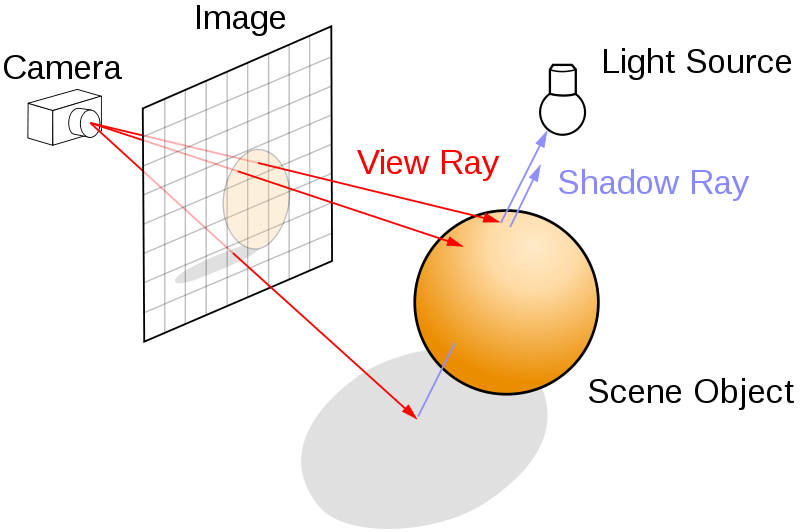
\includegraphics[scale=0.4]{res/ray_tracing.png}
\end{figure}

选定视点位置及一观察屏,从视点到屏上各点发出光线与空间中物体求交.
在交点处根据局部光照模型计算颜色,再递归的计算反射、透射光颜色,混合后显示在屏上.

此程序使用的局部光照模型为Phong模型,其主要公式为\cite{phong}:

\[  I_p = k_ai_a + \sum_{m\in lights} (k_d ( \overrightarrow{L_m} \cdot \overrightarrow{N} i_{m, d} + k_s(\overrightarrow{R_m}\cdot
  \overrightarrow{V})^{\alpha} i_{m, s}))  \]

其中$ k_s, k_d, k_a, \alpha$分别为物体表面该点处的高光系数,漫反射系数,环境光系数,亮度.
$ \overrightarrow{L_m}$为该点指向光源的向量, $ \overrightarrow{N}$为表面法向,
$ \overrightarrow{R_m}$为光源指向该点的光线经理想反射后的指向,
$ \overrightarrow{V}$为视点到表面交点处的向量.

\subsection{几何对象表示及计算}
程序支持了平面、球、三角面片、包围盒四类基本几何物体,
物体都需要各自拥有与光线求交的方法.

\begin{description}
  \item[光线]光线是一条射线,包含一个起始点及方向. 见\verb|include/geometry/ray.hh|
  \item[无穷平面]
    为了计算方便,使用平面法向及平面到原点的距离作为确定平面的方式.
    平面与光线求交时,首先通过光线指向判断是否相交,再通过
    光线在平面法向方向的投影长度计算交点.见\verb|include/geometry/infplane.hh, renderable/plane.cc|

  \item[球]球由球心及半径唯一确定.球与光线求交时,
    利用球心到它在光线所在直线上的投影的距离判断是否相交,在根据投影位置及勾股定理计算交点.
    求交时要考虑光线起始点在球内部的情形,以供计算相对折射率.见\verb|include/geometry/sphere.hh, renderable/sphere.cc|

  \item[三角面片]三角面片用三个顶点坐标存储.
    为了性能,与光线的求交参考了\cite{triangle, triangle_code}的算法及实现,其基本思想是求解满足
    方程
    \[  \overrightarrow{Orig} + t * \overrightarrow{Dir} = x * \overrightarrow{v_1} + y  \overrightarrow{v_2} + (1 - x -
    y)\overrightarrow{v_3}, t > 0, x, y \in (0, 1), x + y \le 1\]
    的$ (t, x, y)$, 在求交时同时能得到交点的重心坐标\footnote{\url{https://en.wikipedia.org/wiki/Barycentric\_coordinate\_system}}
    ,便于之后进行法向插值.见\verb|include/renderable/face.hh, renderable/face.cc|

  \item[轴平行包围盒]
    轴平行包围盒用最小坐标与最大坐标两个向量存储.
    为了效率,包围盒与光线求交部分参考了\cite{aabb}的算法.
    其基本思想是对每个面逐一计算并更新交点.见\verb|geometry/aabb.hh|
\end{description}


\subsection{视图模型}
一个视图应包括视点及屏幕,且应使视点在屏幕的中轴线上.
视图类\verb|View|存储了视点坐标,屏幕中心坐标,屏幕尺寸,屏幕边沿的空间指向,
这样可以方便的进行视图旋转,视图平移,缩放等导航操作.见\verb|include/view.hh, view.cc|

\subsection{KD树}
KD树是一种空间划分树,原本用于在K维空间中快速查找点,可利用在光线追踪中对物体及其包围盒进行索引.
基本方法是,树中每个节点对应一个包围盒,选取一个轴平行平面将包围盒一分为二作为两个子节点,叶节点维护待存储的物体.
与切分面相交的物体在两节点中都应存储.

\subsubsection{建树}
传统的KD树中,按照使两边点的个数尽量接近的原则选取切分平面,这是由于假设了各个点被查询的概率均等.
在光线追踪中,一般采用面积启发式的平面选取方式\cite{kdtree},选取切平面使得
两个子节点的包围盒表面积与包含物体个数的积之和尽量大,这样可以使KD树在查询时效率更高.
但启发式的建树需要枚举切分平面,计算包含物体个数,复杂度较高.
直接的枚举为$ O(n^2)$复杂度,本程序实现了\cite{kdtree}中提供的$ O(n \log^2 n)$算法.
对于20W面片的龙模型\footnote{models/fixed.perfect.dragon.100K.0.07.obj},
采用不同方法单线程建树的用时及在几个固定视角渲染耗时如下(单位: 秒):

\begin{table}[H]
  \begin{threeparttable}

    \begin{tabular}{c|c|c|c|c|c|c}
      \shline
      & 建树 & 视角1 & 视角2 & 视角3 & 视角4 & 视角5 \\ \hline
      二分建树(终止:100层,15个)  & 0.6  & 1.93  & 2.51  & 3.26  & 4.38  & 5.89  \\ \hline
      SAH建树(终止:100层,20个) & 5.41 & 0.29  & 0.37  & 0.45  & 0.59  & 0.78    \\ \hline
      SAH建树(终止:100层,15个) & 7.82 & 0.24  & 0.33  & 0.41  & 0.52  & 0.68    \\ \shline
    \end{tabular}
    \begin{tablenotes}
      \footnotesize
    \item 注: 1.建树时,以树深度及当前节点所管理的物体个数作为建树结束的判定条件.
    \item 2.此实验的视角1为\verb|main.cc|中\verb|test_kdtree()|提供的视角,其余视角由视角1 zoom in依次得到.
    \item 3.可在\verb|lib/kdtree.cc|中通过注释\verb|KDTree::build()|函数中相应代码切换两种建树算法.
    \end{tablenotes}
  \end{threeparttable}
\end{table}

由表可见SAH建树的查询效率有很大提高,但建树缓慢. 建树效率与渲染效率之间存在trade-off,可以通过改变终止条件来调整.

\subsubsection{求交}
求交的基本方法为,递归寻找两子树的最近\underline{物体}的交点,取较近者为结果返回.

实现时,在每个节点处保存了当前节点的两个孩子的切分平面,这样可以预先判断出离
光线较近的包围盒,若与其内物体相交则不用考虑另一包围盒.
使用此方法应注意,若光线与第一个包围盒所管理的物体相交,应确认与最近物体的交点是否被第一个包围盒\underline{包含}.
因为若不包含,则光线首先打到的物体可能并不是此物体,而是第二个包围盒管理的物体.

\subsection{纹理}
一种纹理相当于一个二维坐标到表面属性的映射.
表面属性除Phong模型参数外,还包括了透明度,用于折射判定.
程序实现了均匀纹理、网格纹理、图片纹理三类纹理,并可通过继承\verb|Texture|类进行扩展.

对于一个物体,由其自己管理三维坐标到二维坐标的映射.
对于平面,采用平面上的二维欧式坐标. 球体采用其极坐标.
网格未支持二维纹理,仅可以使用均匀纹理.

\subsection{抗锯齿}
\begin{enumerate}
  \item 使用Beer-Lambert定律,使得光想亮度按传播距离指数衰减,可以有效消除远处纹理密集处的畸形.
    见\figref{first}与\figref{beer}的对比.

  \item 使用全屏抗锯齿(FSAA),对图片整体应用卷积盒$\begin{bmatrix}1 & 2 & 1\\2 & 4 & 2\\1 & 2 & 1\end{bmatrix} $,
    消除直线锯齿的同时使图片模糊,影响视觉效果.

  \item 对每一像素,计算其与周围像素距离平方之和,若小于某一阈值则应用如上卷积盒,略有效果. 见\verb|CVRender::antialias()|
\end{enumerate}

\subsection{软阴影}
对场景中每一点光源,将其替换为点周围的多个密集点光源以模拟面光源的效果,
即可实现软阴影.
效果如\figref{soft}所示. 实现见\verb|Space::add_light()|.

\subsection{景深}
程序中景深的实现方法为,以焦平面作为屏幕,取焦平面与视点之间某处建一感光器平面.
对视点到焦平面的每条光线,取其与感光器的交点,在交点周围随机采多个样本点向
屏幕同一位置发射光线并执行光线追踪


\subsection{小量处理}
有如下情形需要考虑实数运算中的误差.
考虑光线斜射平面的情形,
反射+EPS,

\subsection{网格简化}

\subsection{多线程}
\begin{enumerate}
  \item 对生成图片中每个像素
\end{enumerate}

% File: design.tex
% Date: Sat Jun 22 17:26:42 2013 +0800
% Author: Yuxin Wu <ppwwyyxxc@gmail.com>

\section{项目设计}
项目的目录结构大致如下:
\dirtree{%
  .1 /.
  .2 report/\DTcomment{本报告的\LaTeX 源代码}.
  .2 demo/\DTcomment{一些演示}.
  .2 resource/\DTcomment{程序使用到的外部资源}.
  .2 src/\DTcomment{程序源代码}.
  .3 include/\DTcomment{头文件}.
  .4 geometry/\DTcomment{实现抽象几何对象}.
  .4 renderable/\DTcomment{定义可渲染几何对象}.
  .4 lib/\DTcomment{程序使用的辅助函数定义}.
  .4 material/\DTcomment{实现表面属性及纹理}.
  .4 render/\DTcomment{定义图像渲染}.
  .3 lib/\DTcomment{辅助函数的实现}.
  .4 debugutils.cc.
  .4 utils.cc.
  .4 imagereader.cc.
  .4 Timer.cc.
  .3 renderable/\DTcomment{可渲染几何对象及其渲染相关操作的实现}.
  .4 face.cc.
  .4 mesh.cc.
  .4 plane.cc.
  .4 sphere.cc.
  .3 gui/\DTcomment{图形界面}.
  .4 main.cxx.
  .4 window.cxx.
  .4 window.hh.
  .4 window.ui.
  .4 objviewer.pro.
  .3 kdtree.cc.
  .3 cvrender.cc.
  .3 mesh\_simplifier.cc.
  .3 space.cc.
  .3 static\_const.cc.
  .3 view.cc.
  .3 main.cc.
  .3 Makefile.
  .3 Doxyfile.
}

\subsection{C++类设计}
\begin{enumerate}
  \item 渲染物体相关类的设计

    所有可渲染物体,包括平面、球、面片、网格、KD树,均继承自\verb|Renderable|基类,当其需要与光线求交时,
    通过\verb|Renderable::get_trace()|返回一个\verb|Trace|类的子类对象指针,由
    \verb|Trace|类完成求交相关的操作.一个\verb|Trace|对象相当于一个物体与一条光线的组合.

    \begin{figure}[H]
      \begin{minipage}[b]{0.46\linewidth}
        \centering
        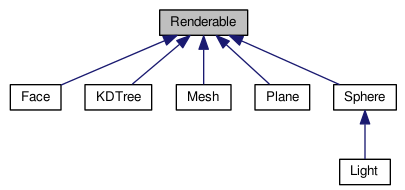
\includegraphics[width=\textwidth]{res/renderable_inherit.png}
      \end{minipage}
      \begin{minipage}[b]{0.46\linewidth}
        \centering
        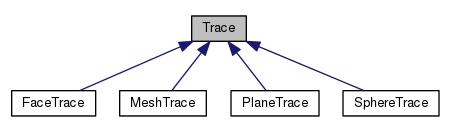
\includegraphics[width=\textwidth]{res/trace_inherit.png}
      \end{minipage}
    \end{figure}

    上图是\verb|Renderable|与\verb|Trace|的继承图,其中\verb|Trace|仅有三个子类是由于\verb|Mesh|返回\verb|FaceTrace|对象指针,
    \verb|KDTree|返回它所管理物体对应的\verb|Trace|对象指针.
    \verb|Renderable|类只有获取物体表面纹理及获取包围盒两种方法,
    \verb|Trace|类包括了判断相交、求交点、求交点法向、交点表面属性、交点前方介质密度等方法.

    这样做的好处是,由\verb|Trace|对象自己管理求交过程的中间结果,保留有用的结果以备其他方法使用.
    如判断是否相交时一些中间结果可能在计算交点距离时使用,交点法向方向有可能被计算纹理映射坐标时使用,
    这些中间结果是每一对$ (物体,光线)$特有的,又不该对外界暴露,因而用\verb|Trace|类将其封装.
    同时,这种设计使得同样的\verb|KDTree|类可以即在网格中又在整个空间中使用,并实现\verb|KDTree|的嵌套.

\end{enumerate}

kdtree

mainwindow

renderable

meshsimplifier

\subsection{视图导航}

\subsection{图形界面}

% File: diary.tex
% Date: Fri Jun 14 12:45:40 2013 +0800
% Author: Yuxin Wu <ppwwyyxxc@gmail.com>
\section{过程记录}
\begin{enumerate}
    \item
首次出现正常的图片. 用了一个$ x-y$平面上的无限大平面及一个点光源。
此时仅仅参考\cite{phong}考虑了基本Phong模型中的漫反射与环境光,已经可以看到左下部分亮度较高,符合预期。

另外,远处的黑白纹理误差较大,不知是不可改进的浮点误差还是我的处理有误。
\begin{figure}[H]
  \centering
  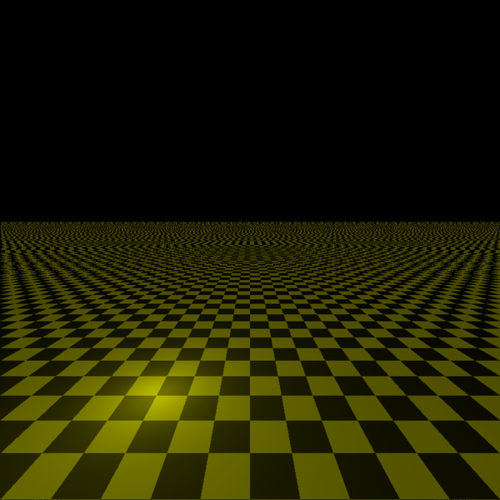
\includegraphics[scale=0.4]{res/first_pic.png}
  \caption{\label{fig:first}}
\end{figure}

\item
依照Beer-Lambert定律\cite{beer}对光线能量进行了按距离的减弱:
\[ E = E_0 e^{distance * density}\]
使得远处的纹理更自然.
\begin{figure}[H]
  \centering
  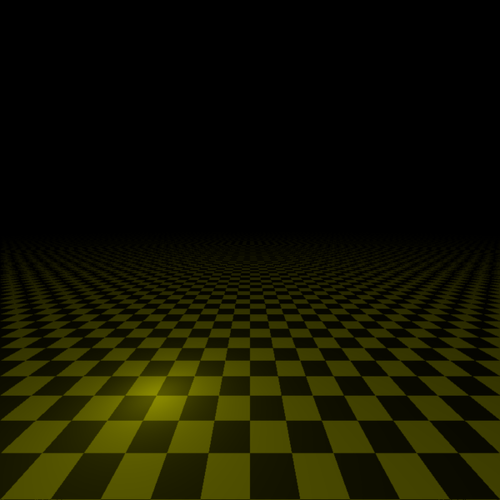
\includegraphics[scale=0.4]{res/plane_with_beer.png}
  \caption{\label{fig:beer}}
\end{figure}

\item

考虑了Phong模型中的高光,并对$ x-y$平面和$ y-z$平面加入了反射系数,有了互相反射的效果,并且
左下部分能够看到高光.打开\verb|-O3|编译开关时,在我的机器上渲染一张$600 \times 600$的图片需要0.39s.
\begin{figure}[H]
  \centering
  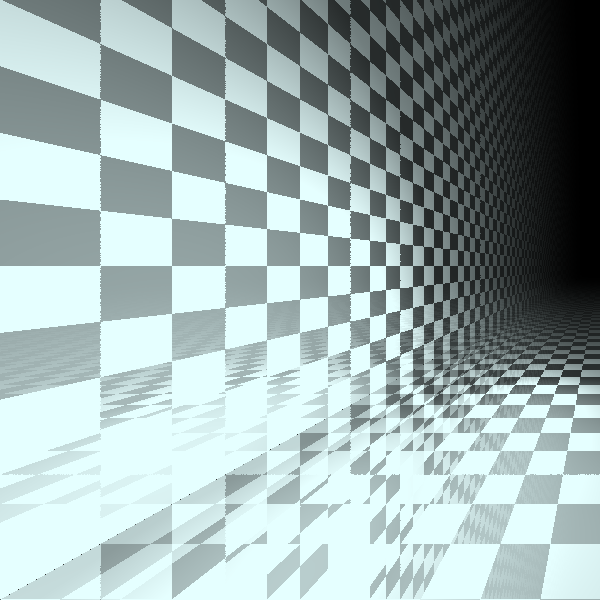
\includegraphics[scale=0.4]{res/specular.png}
  \caption{\label{fig:specular}}
\end{figure}

\item

  使用球模型,可以看到明显的高光效果。同时由于球面\verb|specular|参数高,使得球下部反射了平面。
\begin{figure}[H]
  \centering
  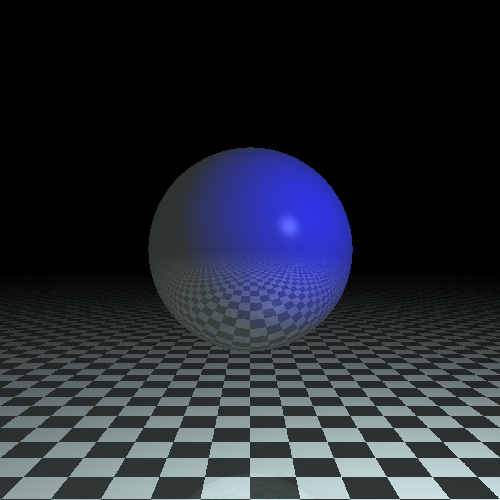
\includegraphics[scale=0.4]{res/ball.png}
  \caption{\label{fig:ball}}
\end{figure}

\item
  对于找到的交点,判断它与光源之间是否被挡住,若被挡住就不计算漫反射和高光. 这样实现了阴影效果.
\begin{figure}[H]
  \centering
  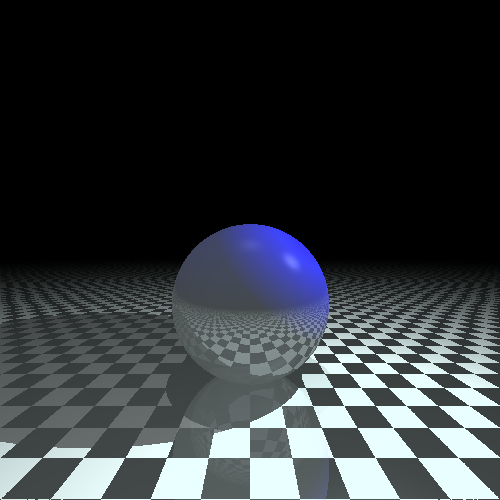
\includegraphics[scale=0.4]{res/shadow.png}
  \caption{\label{fig:shadow}}
\end{figure}

\item 对根据视点及对象生成视图(View)的方案进行修改,以支持视图的旋转,缩放.并利用opencv的key event实现了gui的旋转,缩放控制.
\begin{figure}[H]
  \centering
  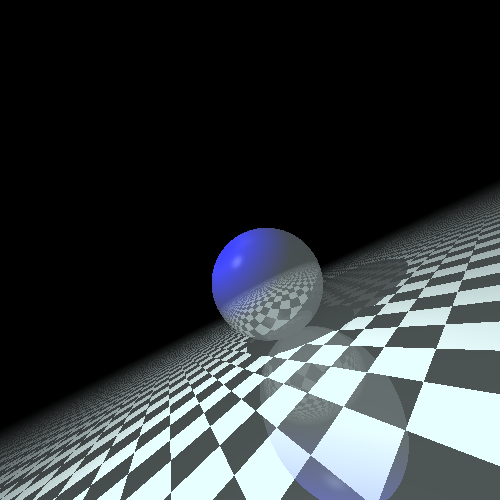
\includegraphics[scale=0.4]{res/rotate.png}
  \caption{\label{fig:rotate}}
\end{figure}

\item 加入了透射功能,依照预定义的介质密度及折射定律计算出射光方向.
\begin{figure}[H]
  \centering
  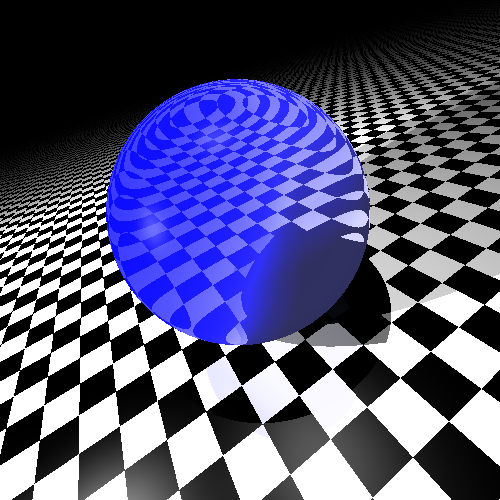
\includegraphics[scale=0.4]{res/transmission.png}
  \caption{\label{fig:transmission}}
\end{figure}

\item 实现了三角面片的渲染,在求交时计算齐次重心坐标,为网格中的法向插值做准备.
\begin{figure}[H]
  \centering
  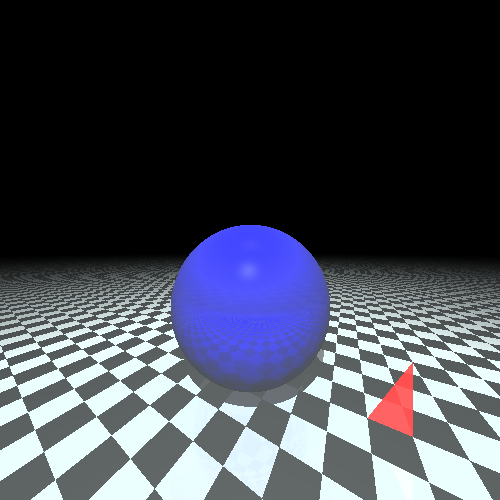
\includegraphics[scale=0.4]{res/face.png}
  \caption{\label{fig:face}}
\end{figure}


\end{enumerate}

\printbibliography

\end{document}

